\chapter{Probabilistic Models} \label{chap:models}

\section*{}

\section{Introduction}

Probabilistic or statistical models represent explicit assumptions about a 
problem domain, in the form of a model. This model usually encompasses random 
variables\footnote{Variable whose value is given by a probability distribution, 
commonly represented by $\Theta$.}, in the form of probability distributions, 
and the relation and dependence between the variables.~\cite{Winn2013}

In the following sections we describe a common way to represent probabilistic models, probabilistic graphical models (PGM) or, simply, graphical models.

\section{Probabilistic Graphical Models}

A PGM is a graph based model where the nodes represent random variables and the 
(directed or undirected) edges represent a conditional dependence between 
variables. An example is shown in figure~\ref{fig:pgm}.

\begin{figure}[h]
	\begin{center}
		\leavevmode
		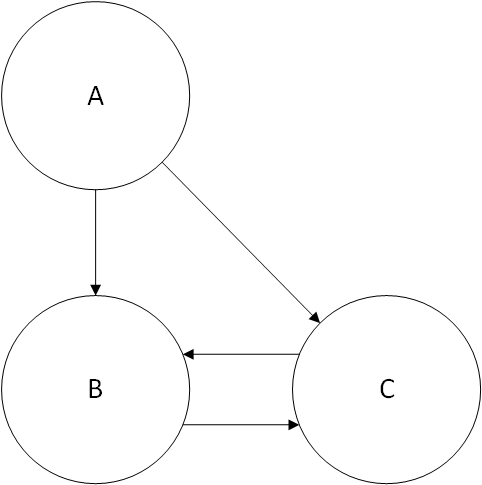
\includegraphics[width=0.36\textwidth]{pgm}
		\caption{Example of a PGM: B and C depend on A, B depends on C and C 
		depends on B.}
		\label{fig:pgm}
	\end{center}
\end{figure}

PGMs and their extensions, where we show some examples of them in the following 
sections, are exceptionally well suited for reasoning and to reach conclusions 
based on available information (both domain expert and data), even in the 
presence of uncertainty. PGMs provide a general framework that allows 
representation, inference and learning on these 
models.~\cite{koller2009probabilistic}

There is extensive research and available literature in this area. Some notable 
examples include, but are not limited to, the books \textit{"Probabilistic 
Graphical Models: Principles and Techniques"} by Daphne Koller and Nir 
Friedman~\cite{koller2009probabilistic} and \textit{"Pattern Recognition and 
Machine Learning"} (Chapter 8: Graphical Models) by Christopher 
Bishop~\cite{bishop2006pattern}. It is also worth mentioning that there is a 
MOOC \footnote{Massive Open Online Course} named \textit{"Probabilistic 
Graphical Models"}, also by Daphne Koller (Stanford), freely available on 
Coursera \footnote{\url{https://www.coursera.org/course/pgm}}.

In the following sections, we describe three important categories of graphical 
models: Bayesian networks, Markov random fields and its extension to hidden 
Markov models. There are plenty of other graphical models however they were 
deemed not relevant enough to be included in this literature review.

\section{Bayesian Networks}

Bayesian networks, also named directed graphical models, is a type of PGM where 
the edges in the graph representation are directed and represent causal 
relationships between random variables or group of random variables (see figure 
\ref{fig:pgm}). This concept was first introduced by Pearl in 
1985~\cite{Pearl1985}, which uses Bayes' conditioning~\cite{bayes1763essay} as 
the basis for updating information.

Bayesian networks follow the Bayesian approach to statistics and probabilities. 
In contrast to classical or physical probability, Bayesian probability (of an 
event) is a person's \textit{degree of belief} in that event 
~\cite{Heckerman1996}. While it may seen that a degree of belief is somewhat 
arbitrary or may lack precision and accuracy, multiple 
authors~\cite{Ramsey1931, Tversky1974, Shachter1988} argue that small 
variations in probability do not have a big influence in the decision making 
process and that measuring beliefs lead to the same rules of probability (which 
can be summarized with the product rule \ref{eq:product} and the sum rule 
\ref{eq:sum}~\cite{MacKay2005}). 

\begin{equation}
P(x, y \mid \mathcal{H}) = P(y \mid x, \mathcal{H}) P(x \mid \mathcal{H}) 
\footnote{$\mathcal{H}$: hypotesis or assumptions the probabilities are based} 
\label{eq:product}
\end{equation}

\begin{equation}
P(x, \mathcal{H}) = \sum_{y}^{} P(x \mid y, \mathcal{H}) P(y \mid \mathcal{H}) 
\label{eq:sum}
\end{equation}

Formally \cite{Pearl:1988:PRI:534975}, a Bayesian network $ B $ represents a 
joint probability distribution (JPD) over a set of variables $ \mathbf{U}$ and 
can be defined by a pair $ B = \langle G, \Theta \rangle $. $ B $ is a DAG 
(directed acyclic graph) where the vertices represent the random variables $ 
X_{1}, ..., X_{n} $. $ \Theta $ represents the set of parameters that quantify 
the network. For each possible value $ x_{i} $ of $ X_{i} $, and $ 
\prod_{x_{i}} $ of $ \prod_{X_{i}} $ (set of parents of $ X_{i} $ in $ G $), it 
contains a parameter $ \theta_{x_{i} \mid \prod_{x_{i}}} = P_{B}(x_{i} \mid 
\prod_{x_{i}}) $. Therefore, the JPD can be defined as

\begin{equation}
P_{B}(X_{1}, ..., X_{n}) = \prod_{i=1}^{n} P_{B}(X_{i} \mid 
\prod\nolimits_{X_{i}}) =
\prod_{i=1}^{n} \theta_{X_{i} \mid \prod_{X_{i}}} \label{eq:jpd}
\end{equation}

which expresses the factorization properties of the JPD. \cite[section 
8.1.]{bishop2006pattern} goes in detail on how to apply the eq \ref{eq:jpd}.

These properties of Bayesian networks make it an excellent tool for expressing 
causal relationships. Heckerman~\cite{Heckerman1996} lists multiple advantages 
of Bayesian networks on modelling and data analysis: ``readily handles 
situations where some data entries are missing'', ``gain understanding about a 
problem domain and to predict the consequences of intervention'', ``ideal 
representation for combining prior knowledge and data'' and ``efficient and 
principled approach for avoiding the overfitting of data''.

Regarding the area of e-commerce specifically, some research has been done 
where Bayesian networks are applied. \cite{Nasambu2014} is an attempt at 
predicting sales in e-commerce using social media data. \cite{Moe2002} also 
proposes a Bayesian based model to predict online purchasing behaviour using 
navigational clickstream data.

\section{Markov Random Fields}

Markov random fields (MRF) or Markov networks are undirected graphical models 
\cite{Kindermann1980} (in contrast to Bayesian networks which are directed and 
acyclic). The nodes still represent variables or group of variables however the 
links do not carry arrows. The concept was originally proposed as the general 
setting for the Ising model\footnote{Ising model: mathematical model of 
ferromagnetism in statistical mechanics}~\cite{Kindermann1980}. Again, 
Bishop~\cite{bishop2006pattern} provides a very good overview of this topic. 

MRFs factorize as

\begin{equation}
p(x_{1}, ..., x_{n}) = \frac{1}{Z} \prod_{C \subset \mathfrak{C}}^{} 
\psi_{C}(x_{C}) \label{eq:markov_factor}
\end{equation}

where $ C $ is a clique\footnote{clique: fully connected subset of vertices} of 
the graph and $ x_{C} $ is the set of variables in that clique, $ Z $ is a 
constant used to normalize the distribution (might be defined for each $ x $), 
$ \psi_{C} $ is a compatibility or potential function~\cite[section 
2.1.2]{Wainwright2008} \cite[section 8.3]{bishop2006pattern}. The equation 
\ref{eq:markov_factor} highlights an important property of MRFs: the Markov 
property or memoryless property. That is, the conditional probability 
distribution of future states depends only on the present state. 

Markov models were shown to be well suited for modelling and predicting 
e-commerce purchasing and user's browsing behaviour \cite{Deshpande2001}. The 
same article states ``there will be cases in which a user’s Web site
browsing process is not Markovian and, in these cases, such an assumption will
lead to inaccurate modeling'' however this claim is groundless.

\section{Hidden Markov Models}

Hidden Markov models (HMMs) are a PGM with unobserved or hidden states. They 
are considered a dynamic Bayesian network\footnote{dynamic Bayesian network: 
Bayesian networks adapted with time steps}. They have been originally defined 
in the 60s by Baum and colleagues \cite{Baum1966}. \cite{Rabiner1989} defines 
HMMs as ``the resulting model (...) is a doubly embeded stochastic process that 
is not observable, but can only be observed though another set of stochastic 
processes that produce the sequence of observations.''.

A common example found in literature is the Coin Toss Model~\cite{Rabiner1989}: 
imagine someone on one side of a curtain performing a coin (or multiple coin) 
tossing experiment. The other person will not tell us about what she is doing, 
only the outcome of each coin flip (heads or tails). Multiple HMMs can be built 
to explain the coin toss outcomes, i.e, assuming that one, two or more biased 
coins are being used in the experiment. The figure \ref{fig:hmm_coins} is a 
possible model that can account to 3 coins being tossed.

\begin{figure}[h]
    \begin{center}
        \leavevmode
        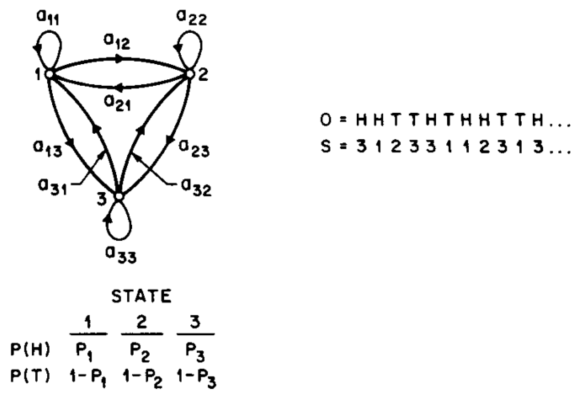
\includegraphics[width=0.56\textwidth]{hmm_coins}
        \caption{Example of a 3-coin model \cite{Rabiner1989}}
        \label{fig:hmm_coins}
    \end{center}
\end{figure}

A HMM is characterized by the following:
\begin{itemize}
    \item $ N $ which is the number of states in the model where individual 
    states are represented by $ S = \{ S_{1}, ..., S_{N} \} $ and the state at 
    time $ t $ is $ q_{t} $;
    \item $ M $ which is the number of distinct observation symbols per state 
    (individual symbols are represented by $ V = \{V_{1}, ..., V_{M} \} $);
    \item $ A = \{ a_{i, j} \} $, the state transition probability 
    distribution where
    \begin{equation}
    a_{ij} = p(q_{t+1} = S_{j} \mid q_{t} = S_{i}), 1 \leq i, j \leq N
    \end{equation}
    \item $ B = \{ b_{j}(k) \} $, the observation symbol probability 
    distribution in state $ j $:
    \begin{equation}
    b_{j}(k) = p(v_{k}~at \mid q_{t} = S_{j}), 1 \leq j \leq N, 1 \leq k 
    \leq M
    \end{equation}
    \item Finally, $ \pi = \{ \pi_{i} \} $, the initial state distribution:
    \begin{equation}
    \pi_{i} = p(q_{1} = S_{i}), 1 \leq i \leq N
    \end{equation}
\end{itemize}

The formal model can be summarized as $ \lambda = (A, B, \pi) 
$~\cite{Rabiner1989}.

Multiple algorithms have been studied and applied to HMMs: for inference, the 
forward algorithm, forward-backward algorithm \cite{baum1967inequality} or the 
Viterbi algorithm \cite{forney2005viterbi, martin2000speech}. Regarding 
learning, the algorithm Baum-Welch \cite{Baum1966, baum1967inequality} can be 
used.

Regarding e-commerce and web user behaviour there is some research done. 
\cite{Xie2009}~explains how to use a hidden semi-Markov model to detect 
anomalies on user browsing behaviour. \cite{Anderson2002}~describes very 
briefly a relational hidden Markov model for the behaviour of web site users, 
in order to improve predictions and personalization of websites.

\section{Summary}

In this section we reviewed the literature for graphical models. They provide a 
tool of excellence to model real world phenomena, enabling decision making 
under uncertainty and noisy observations.

There are multiple categories of graphical models however we focused on 
Bayesian and Markov networks and hidden Markov models, due to their 
applicability in the work at hand (in chapter \ref{chap:method} we will define 
how PGMs can be applied).
